%%%%%%%%%%%%%%%%%%%%%%%%%%%%%%%%%%%%%%%%%%%%%%%%%%%%%%%%%%%%%%%%%%%%%%%%
%     LaTeX source code to approximate a Draft NIST Technical report
%	  Instructions for authors: tinyurl.com/techpubsnist 
%	DOI watermark will be added on final PDF
% 	Developed by K. Miller, kmm5@nist.gov 
%	Last updated: 22-March-2019
%%%%%%%%%%%%%%%%%%%%%%%%%%%%%%%%%%%%%%%%%%%%%%%%%%%%%%%%%%%%%%%%%%%

%%%%%%%%%%%%%%%%%%%%%%
% Template further altered by Armen Amirkhanian
% for use with UA lab courses in an effort to 
% have a standardized format for lab documents
% Last update 9-April-2020
%
% TODO:
% --Get the appendices to dynamically link, tocloft causes problems
%%%%%%%%%%%%%%%%%%%%%%

\documentclass[12pt]{article}
\usepackage{amsmath}
\usepackage{amsfonts}   % if you want the fonts
\usepackage{amssymb}    % if you want extra symbols
\usepackage{graphicx}   % need for figures
\usepackage{xcolor}
\usepackage{bm}
\usepackage{secdot}		
\usepackage{mathptmx}
\usepackage{float}
\usepackage[utf8]{inputenc}
\usepackage{textcomp}
\usepackage[hang,flushmargin,bottom]{footmisc} % footnote format
\usepackage{xspace}
%\usepackage{lineno}
\usepackage{ragged2e}
\usepackage{parskip}

\usepackage{tikz}
\usetikzlibrary{shapes.geometric, arrows}
\tikzstyle{startstop} = [rectangle, rounded corners, minimum width=2cm, minimum height=1cm,text centered, draw=black, fill=red!20]
\tikzstyle{arrow} = [thick,->,>=stealth]

\usepackage{titlesec}
\titleformat{\section}{\normalsize\bfseries}{\thesection.}{1em}{}	% required for heading numbering style
\titleformat*{\subsection}{\normalsize\bfseries}

\usepackage{tocloft}	% change typeset, titles, and format list of appendices/figures/tables
\renewcommand{\cftdot}{}	
\renewcommand{\contentsname}{Table of Contents}
\renewcommand{\cftpartleader}{\cftdotfill{\cftdotsep}} % for parts
\renewcommand{\cftsecleader}{\cftdotfill{\cftdotsep}}
\renewcommand\cftbeforesecskip{\setlength{4pt}{}}
\addtolength{\cftfignumwidth}{1em}
\renewcommand{\cftfigpresnum}{\figurename\ }
\addtolength{\cfttabnumwidth}{1em}
\renewcommand{\cfttabpresnum}{\tablename\ }
\setlength{\cfttabindent}{0in}    %% adjust as you like
\setlength{\cftfigindent}{0in} 

\usepackage{enumitem}         % to control spacing between bullets/numbered lists

\usepackage[numbers,sort&compress]{natbib} % format bibliography 
\renewcommand{\bibsection}{}
\setlength{\bibsep}{0.0pt}

\usepackage[hidelinks]{hyperref}
\hypersetup{
	colorlinks = true,
urlcolor ={blue},
citecolor = {.},
linkcolor = {.},
anchorcolor = {.},
filecolor = {.},
menucolor = {.},
runcolor = {.}
pdftitle={},
pdfsubject={},
pdfauthor={},
pdfkeywords={}
}
\urlstyle{same}

\usepackage{epstopdf} % converting EPS figure files to PDF

\usepackage{fancyhdr, lastpage}	% formatting document, calculating number of pages, formatting headers
\setlength{\topmargin}{-0.5in}
\setlength{\headheight}{39pt}
\setlength{\oddsidemargin}{0.25in}
\setlength{\evensidemargin}{0.25in}
\setlength{\textwidth}{6.0in}
\setlength{\textheight}{8.5in}

\usepackage{caption} % required for Figure labels
\captionsetup{font=small,labelfont=bf,figurename=Fig.,labelsep=period,justification=raggedright} 

%%%%%%%%%%% !!!!!REQUIRED - FILL OUT METADATA HERE !!!!!!!! %%%%%%%%%%%%%%
%%%%%%%%%%%%%%%%%%%%%%%%%%%%%%%%%%%%%%%%%%%%%%%%%%%%%%%%%%%%%%%%%%%%%%%%%%
\newcommand{\CourseNum}{CE340}
\newcommand{\CourseName}{Geotechnical Engineering}
\newcommand{\LabTitle}{Sieve Analysis and Hydrometer Testing}
\newcommand{\LastUpdate}{Summer 2020}

%%%%%%%%%%%%%%%%%%%%%%%%%%%%%%%%%%%%%%%%%%%%%%%%%%%%%%%%%%%%%%%%%%%%
%   	BEGIN DOCUMENT 
%%%%%%%%%%%%%%%%%%%%%%%%%%%%%%%%%%%%%%%%%%%%%%%%%%%%%%%%%%%%%%%%%%%%
\begin{document}
	\urlstyle{rm} % Format style of \url   
%\linenumbers
\begin{titlepage}
\begin{flushright}
\LARGE{\textbf{\CourseNum{} -- \CourseName}}\\
\vfill
\Huge{\textbf{\LabTitle}}\\
    \vfill
%%%%%%%%%%%%%%%%%%%%%%%%%%%%%%%%%%%%%%%%%%%%%%%%%%%%%%%%%%%%%%%%%%%%
%	Authors - add complete list of authors, affiliations will be 
%   added on title page
%%%%%%%%%%%%%%%%%%%%%%%%%%%%%%%%%%%%%%%%%%%%%%%%%%%%%%%%%%%%%%%%%%%%
    \large Dr. Armen Amirkhanian, P.E.\\
\vfill
%%%%%%%%%%%%%%%%%%%%%%%%%%%%%%%%%%%%%%%%%%%%%%%%%%%%%%%%%%%%%%%%%%%%
%	The DOI is automated based on metadata.	
%%%%%%%%%%%%%%%%%%%%%%%%%%%%%%%%%%%%%%%%%%%%%%%%%%%%%%%%%%%%%%%%%%%%
\normalsize This work is licensed under the Creative Commons Attribution-ShareAlike 4.0 International License. To view a copy of this license, visit:
\href{http://creativecommons.org/licenses/by-sa/4.0/}{http://creativecommons.org/licenses/by-sa/4.0/}.


\includegraphics[width=0.07\textwidth]{cc.eps}

\includegraphics[width=0.07\textwidth]{by.eps}

\includegraphics[width=0.07\textwidth]{sa.eps}
\vfill


\includegraphics[width=0.3\linewidth]{Logo.eps}\\ 
 
  
\end{flushright}
\end{titlepage}

\begin{titlepage}
\begin{center}
\normalsize 
Certain commercial entities, equipment, or materials may be identified in this document in order to describe an experimental procedure or concept adequately. Such identification is not intended to imply recommendation or endorsement by The University of Alabama or the listed authors, nor is it intended to imply that the entities, materials, or equipment are necessarily the best available for the purpose.\\
\vfill
Any opinions or recommendations are solely those of the authors and do not represent the official view or policy of The University of Alabama.
\end{center}
\begin{flushright}
\vfill
\normalsize 
This document was last updated in \textbf{\LastUpdate} and should contain \textbf{\pageref{LastPage}} pages of content exclusive of these title pages, abstract, and other front matter. If the document appears to be incomplete, please contact the author(s).\\
\vfill
Take chances, make mistakes, get messy!\\
\textit{Ms. Frizzle}
\end{flushright}
\end{titlepage}
%%%%%%%%%%%%%%%%%%%%%%%%%%%%%%%%%%%%%%%%%%%%%%%%%%%%%%%%%%%%%%%%%%%%
%   Start front matter - page number starts with "i"
%%%%%%%%%%%%%%%%%%%%%%%%%%%%%%%%%%%%%%%%%%%%%%%%%%%%%%%%%%%%%%%%%%%%
\pagenumbering{roman}
\section*{Abstract}
\normalsize A soil's gradation characteristics are one of the fundamental properties that can describe a material in sufficient detail to classify and utilize the material in a wide variety of applications. Numerous agencies and code bodies (i.e. state highway agencies (SHAs), International Building Code (IBC), American Concrete Institute (ACI), Superpave, etc.) all use gradations to ensure materials such as backfill, structural fill, and pavement mixtures have adequate strength and durability. The gradation itself is a description of the amount of material present at a set or range of specific sizes. For example, part of a gradation analysis may determine that a soil sample has particles that are 65\%, by weight, smaller than 0.5 inches.

There are numerous methods to characterize a soil or aggregate gradation. This lab exercise will describe two of the most common methods: sieve analysis and hydrometer testing. The sieve analysis procedure physically separates the sample on successively smaller sieves. The weight of material retained on each sieve is then measured and a gradation is calculated. The hydrometer test indirectly characterizes the gradation of materials that are extremely small (i.e. particle size is less than 75 $\mu$m). In this method, the sample is blended in a high-shear mixer and then allowed to settle out over time. The change in density is measured over time and from Stokes Law, the particle sizes can be calculated.\\

\vfill
\section*{Keywords}
\normalsize fineness modulus; gradation; hydrometer; sieve analysis.\\
\pagebreak
%%%%%%%%%%%%%%%%%%%%%%%%%%%%%%%%%%%%%%%%%%%%%%%%%%%%%%%%%%%%%%%%%%%%
%   Table of Contents is required
% 	List of Tables & Figures required if more than 5 tables/figures
%%%%%%%%%%%%%%%%%%%%%%%%%%%%%%%%%%%%%%%%%%%%%%%%%%%%%%%%%%%%%%%%%%%%
\begin{center}
\tableofcontents
\pagebreak
\listoftables
\listoffigures
\end{center}
\pagebreak
\section*{Required Specifications}
The following specifications are required to complete this laboratory exercise:
\begin{description}
\item[ASTM C136] Standard Test Method for Sieve Analysis of Fine and Coarse Aggregates
\item[ASTM D6913] Standard Test Methods for Particle-Size Distribution (Gradation) of Soils Using Sieve Analysis
\item[ASTM D7928] Standard Test Method for Particle-Size Distribution (Gradation) of Fine-Grained Soils Using the Sedimentation (Hydrometer) Analysis
\item[ASTM E11] Specification for Woven Wire Test Sieve Cloth and Test Sieves
\end{description}

The following specifications are optional, but they are listed here in the event more information is needed to complete the laboratory exercise:
\begin{description}
\item[ASTM D6026] Standard Practice for Using Significant Digits in Geotechnical Data
\item[ASTM E100] Specification for ASTM Hydrometers
\end{description}
\pagebreak
%%%%%%%%%%%%%%%%%%%%%%%%%%%%%%%%%%%%%%%%%%%%%%%%%%%%%%%%%%%%%%%%%%%%
%   Start body of text - page number starts with "1"
%%%%%%%%%%%%%%%%%%%%%%%%%%%%%%%%%%%%%%%%%%%%%%%%%%%%%%%%%%%%%%%%%%%%
\section{Sieve Analysis Procedure}
\label{sec:intro}
\pagenumbering{arabic}
\normalsize 
A sieve\footnote{Pronounced ``sive''like ``give''; not ``seeve'' like ``grieve''. Surest way to look like a rookie in front of your new boss!} analysis is a process in which the soil material is separated into various sizes by using a combination of sieves. A sieve is typically a round or rectangular frame that has a wire cloth inside it. This cloth is a precisely woven material that has a specific opening size as outlined in ASTM E11. Multiple sieves are stacked in descending size to perform the analysis. This sieve stack is then physically or mechanically agitated to ensure all the particles have a chance to fall through the openings in the wire cloth. Finally, the amount retained on each sieve is weighed and the results can be plotted.

\subsection{Objectives}
\label{ssec:headingscap}
At the completion of this lab exercise, you will have satisfied the following objectives:
\begin{enumerate}
    \item Perform sieve analysis on a silty-clayey soil material
    \item Perform sieve analysis on a sandy soil material
    \item Perform sieve analysis on a coarse aggregate
    \item Perform calculations necessary to determine the requisite gradation properties
    \item Construct gradation chart of three aforementioned materials down to a \#200 (75 $\mu$m) sieve size
\end{enumerate}

\subsection{Learning Outcomes}
At the completion of this lab exercise, you should be able to:
\begin{itemize}
    \item understand what a sieve is and how a sieve stack is utilized to obtain gradation information
    \item perform calculations necessary to characterize the gradation of a sieve analysis
    \item understand how to interpret a gradation chart and fineness modulus values when provided with specification requirements
    \item present information on gradations in a useful and professional manner
\end{itemize}

\pagebreak
\subsection{Procedure}
The sieve analysis procedure is divided into three parts: preparation, execution, and analysis. Given the importance placed on accurate sieve analyses, it is critical to keep accurate notes and follow steps carefully and accurately. When an engineer presents their stamped work to a client, a phrase similar to ``the values were determined in accordance with ASTM D6913'' will be included. This is not a generic phrase! You are legally stating you followed \textbf{all} of the requirements outlined in the specification. If you skipped a step, and the client found out or suspected the numbers were off, they would have legal standing to challenge your results. If you did follow the specification exactly, then you can correctly use that phrase. If you did not, one alternative is ``the values were determined using generally accepted procedures such as ASTM D6913 and others''. However, if you were a client, would you want a firm to follow specifications exactly or one that gets most of it?

We are going to run two sieve analysis procedures: ASTM C136 and ASTM D6913. They are fairly similar with a few specific differences. The ASTM C136 procedure is typically used on aggregate sources for concrete and asphalt mixtures. It is a simpler procedure because it assumes there are no significant amount of fines\footnote{Fines are usually considered particles smaller than the \#200 sieve (75 $\mu$m).} present in the sample that are plastic\footnote{The topic of plasticity is covered in the companion Atterberg Limits laboratory exercise.}. The ASTM D6913 is better suited for soils with significant amount of fines as the test method specifies procedures to separate the fine particles.

\subsubsection{Preparation}
We have three materials that need to be characterized: silty-clayey soil, sandy soil, and coarse aggregate. The silty-clayey soil will be characterized with ASTM D6913 and the sandy soil and coarse aggregate will be characterized with ASTM C136. The actual sieve sizes we use are minimally specified; that is, the specification outlines the minimum sizes we should use but we could add additional sizes depending on our objective. For this exercise, we will stick with the minimum requirements.

The minimum requirements for ASTM C136 are in \S8.2\footnote{The goofy looking \S{} symbol means ``section''; so this is telling you to look at section 8.2 in the specification.} and simply state that the minimum sieves are those specified by the client or agency. For this laboratory exercise, the required sieves are: 19 mm, 9.5 mm, \#4, \#8, \#16, \#30, \#50, \#100. These particular sieves are chosen so that the fineness modulus can be calculated for the sandy soil sample as described in ASTM C136 \S9.2.

The minimum requirements for ASTM D6913 are in \S6.1.1 and Table 1 within the standard. Because this method is designed for soil materials that can have a wide range of particle sizes, there are significantly more sieves. So many, in fact, that we split the test into two ``runs''.

The sieve analysis procedure is done on a weight-basis (i.e. all calculations are done using weights, not volumes). We are going to be recording a variety of weights\footnote{For this laboratory exercise, weight and mass are used interchangeably. Since the materials being measured are not moving and we assume the gravitational force exerted on them is constant, we can safely make this assumption. Additionally, we are not calculating the force exerted by the materials. In other parts of this course, we will distinguish between weight and mass using gravity.} and it is important to prepare a worksheet prior to lab to aid in collecting the necessary data.

To aid us in creating a worksheet, let's think about what we want at the end of the test: weight of aggregate sitting on each sieve. Well, we could shake the sieve stack, separate the sieves, then dump the amount in each sieve on the scale and measure it. However, with the smaller sieve sizes, it is really difficult to get all the particles out of the woven cloth. Thus, our measurements are likely to be off, and in some cases significantly off! So, we need to first measure the weight of the empty sieves, run the sieve analysis, then weigh the sieve with the retained material. We can then subtract the weight of the empty sieve and obtain the retained mass! An example data collection worksheet is shown in Appendix A.

We will also need the starting weight of the material. It is possible to sieve too much material and get erroneous results. Fortunately, both specifications outline the maximum allowable on the individual sieves and total starting weights. For ASTM C136, this starting sample weight information is found in \S7.3 and \S7.4 for fine aggregate and coarse aggregate, respectively. The overload weight for each sieve for ASTM C136 is found in \S8.3. For ASTM D6913, this starting sample weight information is found in \S10.2. The overload weight for each sieve for ASTM D6913 is found in \S11.3.

\subsubsection*{Preparation Checklist}
\begin{itemize}
    \item Obtain correct sieves, note any missing sieves
    \item Weigh empty sieves
    \item Determine minimum weight of material needed for test
    \item Weigh starting sample
\end{itemize}

\subsubsection{Execution}
We are now ready to run the sieve analysis. For both specifications, the end goal is to separate the particles into their individual sizes. Both specifications describe manual and mechanical agitation methods to expedite the sieving process. For this laboratory exercise, we will utilize mechanical shaking methods for both procedures.

Neither specification outlines a precise time to shake the sieves. This is because soil materials do not sieve equally. Both specifications outline trial procedures to use to determine the amount of time to sieve a sample. A typical shaking time for ASTM C136 materials is 5--10 minutes whereas ASTM D6913 materials have shaking times around 15--20 minutes. For this laboratory exercise, the ASTM C136 test will be run with a shaking time of 7 minutes and the ASTM D6913 test will be run with a shaking time of 15 minutes.

Because the sieves are expensive and damage can occur if they are not loaded into the sieve shaker properly, the instructor will assist you with this process. Make note if the correct shaking time is used.

After the shaking period has ended, the sieve stack will be removed from the shaker. The next step is one of the hardest steps for this entire process: separating the sieve stacks without spilling material. The sieves have been pounded together and particles have wedge themselves in-between the sieves. The instructor will demonstrate the technique to use to correctly separate the sieves.

With the sieves now separated, they can be individually weighed. If material was lost during the separation process, note it in your report but perform the calculations with the values you measure. Do not attempt to guess how much material was lost. You may notice that some sieves appear empty. You should still weigh them. If there was a particle stuck in the mesh prior to the shaking process and it came loose, you will see a decrease in the apparent mass, indicating you were not careful in the preparation of the test.

\subsubsection*{Execution Checklist}
\begin{itemize}
    \item Select correct shaking time for material being sieved
    \item Carefully separate sieve stack after shaking period
    \item Weigh individual sieves
\end{itemize}

\subsubsection{Analysis}
We should now have enough data to calculate and plot the gradation of the three materials characterized in the laboratory exercise. The first thing to do is calculate the mass of material on each sieve. You have likely figured out by now we simply subtract the empty weight of the sieve from the weight of the sieve with the material in it. At this point, the individual masses should be summed to see how close it is to the original starting mass. This is a very important check as any discrepancy would indicate that material was lost during the test. The maximum allowable loss of material is 0.3\% for ASTM C136 procedures. Interestingly, ASTM D6913 does not specify a maximum allowable loss.

With individual retained weights and the summed weight, we can calculate the percentage retained on each sieve. With the retained percentages on each sieve, we can then calculate a cumulative, or running total, of percentage retained. Finally, the cumulative passing is simply 100\% minus the cumulative retained. An example dataset is shown in Table \ref{tab:gradation} and can be used to check the spreadsheet you develop for this laboratory exercise. Note that the \#200 sieve value for cumulative retained goes to one decimal place. This is required by ASTM C136 \S10.2. There are a couple of checks one can do to ensure the calculations are correct:
\begin{itemize}
    \item Cumulative retained must always end at 100\% at the pan.
    \item Cumulative retained values must always increase from sieve to sieve down the stack.
    \item Cumulative passing must always end at 0\% at the pan.
    \item Cumulative passing values must always decrease from sieve to sieve down the stack.
\end{itemize}

\begin{table}[H]
\centering
\caption{Example calculations of gradation data which can be used to check your spreadsheet.}
\label{tab:gradation}
\begin{tabular}{@{}cccccc@{}}
\hline
Sieve   & \begin{tabular}[c]{@{}c@{}}Sieve\\ {[}g{]}\end{tabular} & \begin{tabular}[c]{@{}c@{}}Sieve\\ + Agg\\ {[}g{]}\end{tabular} & \begin{tabular}[c]{@{}c@{}}Agg\\ {[}g{]}\end{tabular} & \begin{tabular}[c]{@{}c@{}}Retained\\ {[}\%{]}\end{tabular} & \begin{tabular}[c]{@{}c@{}}Cuml.\\ Retained\\ {[}\%{]}\end{tabular} \\ \hline
No. 4   & 721.51    & 744.87     & 23.36     & 3     & 3  \\
No. 8   & 436.15    & 487.45     & 51.30     & 6     & 9  \\
No. 16  & 393.18    & 449.90     & 56.72     & 6     & 15 \\
No. 30  & 350.82    & 455.55     & 104.73    & 11    & 26 \\
No. 50  & 558.74    & 959.93     & 401.19    & 44    & 70 \\
No. 100 & 317.71    & 565.17     & 247.46    & 27    & 97 \\
No. 200 & 248.41    & 269.95     & 21.54     & 2.4   & 99.4\\
Pan     & 355.94    & 365.46     & 9.52      & 1.0   & 100\\ \hline
\end{tabular}
\end{table}

The spreadsheet you develop for this laboratory exercise should be able to automatically calculate the gradation with the only inputs being the empty sieve weight and sieve weight with retained material. All other calculations should be automatic and done with equations in the spreadsheet.

This fineness modulus is typically used for daily quality control at a quarry or ready-mix plant to monitor the aggregate sources for changes. In some cases, agencies will specify a minimum and maximum fineness modulus value for a project. A lot of times, the fineness modulus is abbreviated FM and is typically only used on fine aggregates, but can be used on coarse aggregates. As previously mentioned, the specifics of the calculation are in ASTM C136 \S9.2. Given the example data below, the calculated FM would be 2.76 (Table \ref{tab:FM}).

\begin{table}[H]
    \centering
        \caption{Example dataset for FM calculation.}
    \label{tab:FM}
    \begin{tabular}{ccc}
\hline
Sieve Size & Ret., \% & Cuml. Ret., \% \\ \hline
3/8" & 0 & 0 \\
\#4 & 2 & 2 \\
\#8 & 13 & 15 \\
\#16 & 25 & 40 \\
\#30 & 15 & 55 \\
\#50 & 22 & 77 \\
\#100 & 10 & 87 \\
\#200 & 10 & 97 \\
Pan & 3 & 100 \\ \hline
\end{tabular}
\end{table}

\subsubsection*{Analysis Checklist}
\begin{itemize}
    \item Calculate cumulative retained and cumulative passing for all three soil material sources
    \item Calculate the FM of the sandy soil sample
\end{itemize}

\subsection{Summary}
We have successfully planned, executed, and analyzed the results of a sieve analysis on three different materials using two different ASTM specifications. This relatively straightforward process forms the basis of numerous engineering endeavors. All disciplines within civil engineering utilize gradation information for hazardous waste diffusion, concrete mixture design, slope stability, etc.

However, the test methods used to obtain the gradation data are sometimes insufficient. You may have noticed that the silty-clayey soil sample had a significant amount of material that passed the \#200 sieve. We need a method to evaluate the gradation to an even smaller particle size. Why? We need to know how much clay and silt we have in our sample as these materials can significantly affect the behavior we encounter in the field.

\pagebreak
\section{Hydrometer Testing Procedure}
The hydrometer testing procedure is an interesting procedure that indirectly measures the particle sizes of a soil sample that are smaller than the \#200 sieve (75 $\mu$m). The keyword here is indirect measure. While it is possible to purchase sieves that have incredibly small openings, they are, as expected, incredibly expensive! Not to mention extremely fragile and easily clogged.

A hydrometer solves this issue as it is simple, requires no batteries, and maintains calibration relatively well. When we place the hydrometer into a milkshake of soil sample, it will float to a certain level, due to the density of the solution. As the ``milkshake'' settles out, the density changes and the hydrometer slowly floats to a different level. 

This is where Stokes' Law comes into play. We first make several assumptions to use Stokes' Law: smooth, perfectly round particles and the particles do not interact with one another. For certain soils, this assumption can be quite a bad one to make. But we do not have a much better option when it comes to the cost and ease of running the hydrometer test. With those assumptions, Stokes' Law is given by Eq. (\ref{eq:stokeslaw}):

\begin{equation}
    F_d=6\pi\mu R\nu
    \label{eq:stokeslaw}
\end{equation}

where:
\begin{description}
\item[$F_d=$] friction force between particle and fluid
\item[$\mu=$] dynamic viscosity
\item[$R=$] radius of particle
\item[$\nu=$] velocity of fluid or particle
\end{description}
However, Eq. (\ref{eq:stokeslaw}) is not useful for a hydrometer analysis. We are only measuring density changes! If we do some rearranging and most importantly, assume the particles are falling at their terminal velocity within the fluid, we get a more useful form of Stokes' Law given by Eq. (\ref{eq:terminalstokeslaw}):

\begin{equation}
    \nu=\dfrac{2\left(\rho_p-\rho_f\right)gR^2}{9\mu}
    \label{eq:terminalstokeslaw}
\end{equation}

where:
\begin{description}
\item[$\rho_p=$] mass density of particle
\item[$\rho_f=$] mass density of fluid
\item[$g=$] acceleration due to gravity
\end{description}
Almost there! We rearrange Eq. (\ref{eq:terminalstokeslaw}) to its final form which is in terms of diameter of particle\footnote{We want diameter over radius because our normal sieve analysis is giving us the particle diameter.}. The final form of the equation used in ASTM D7928 is Eq. (\ref{eq:modASTM_Eq11}):

\begin{equation}
    D=\sqrt{\dfrac{18\mu\nu}{\rho_f g\left(\rho_p-1\right)}}
    \label{eq:modASTM_Eq11}
\end{equation}

where:
\begin{description}
\item[$D=$] diameter of particle
\end{description}
The actual equation in ASTM D7928, as you will see when you perform the calculations, is slightly different than Eq. (\ref{eq:modASTM_Eq11}) in that the particle velocity, $\nu$, is calculated as the time it takes a particle to fall from an effective depth.

\subsection{Objectives}
At the completion of this lab exercise, you will have satisfied the following objectives:
\begin{enumerate}
    \item Perform a hydrometer test on a silty-clayey soil material
    \item Perform a hydrometer test on a sandy soil material
    \item Perform the calculations necessary to determine the gradation values smaller than the \#200 (75 $\mu$m) sieve
    \item Construct a gradation chart of the two aforementioned materials over the complete range of particle sizes (i.e. combine the sieve analysis and hydrometer analysis)
\end{enumerate}

\subsection{Learning Outcomes}
At the completion of this lab exercise, you should be able to:
\begin{itemize}
    \item understand how Stokes' Law is applied to soil gradation measurements
    \item perform calculations associated with hydrometer measurements to determine gradation values
    \item understand how to combine sieve analysis and hydrometer testing values to form a complete gradation of a soil material
    \item present information on gradations in a useful and professional manner
\end{itemize}

\pagebreak
\subsection{Procedure}
The hydrometer testing procedure is divided into three parts: preparation, execution, and analysis. The testing procedure is relatively straightforward, however, unlike the sieve analysis procedure, it is easier to make measurement errors. If you brew your own beer or are picky with your engine coolant blend ratio, you may already be familiar with how to use a hydrometer and how difficult it can be to actually observe the reading on it.

This test is also extremely sensitive to temperature changes. Recall from Eq. (\ref{eq:modASTM_Eq11}) that there is a viscosity term, $\mu$. This is an important consideration and the test method attempts to minimize the effects of temperature.

\subsubsection{Preparation}
We have two materials to be analyzed: a silty-clayey soil and a sandy soil. If we read ASTM D7928 \S1.2, it states that clean sands cannot be effectively characterized with this method. We will see if our sandy soil has enough fines to be characterized with the hydrometer test method.

The minimum sample weight we need is specified in ASTM D7928 \S3.2.4 with the \#10 (2 mm) sieve used as the separation sieve. The other equipment, meeting the requirements of ASTM D7928, are provided for you. It is important for you to note the hydrometer type (either 151H or 152H) as each one measures values in different units.

The sample itself is usually in some sort of moist condition. The hydrometers we will use can only ``handle'' a certain amount of soil in solution. It is also important to keep the sample sufficiently sealed as you prepare to execute the procedure\footnote{See Note 9 in \S9.1 for why.}. So, if we are weighing a moist sample, the weight we record will be some amount of solids (i.e. the soil) and some amount of water. The 151H hydrometer can handle 45 g of solids and the 152H hydrometer can handle 55 g of solids. The ASTM D7928 specification provides an equation to estimate the amount of moist soil we can add to get close to the capacities of the hydrometers and is shown\footnote{The variable names have been simplified compared to those listed in ASTM D7928 \S9.5.} in Eq. (\ref{eq:moistureestimate}):

\begin{equation}
    M=H_c\times \left(\dfrac{100}{P_{200}}\right)\times \left(1+\left(\dfrac{w_c}{100}\right)\right)
    \label{eq:moistureestimate}
\end{equation}

where:
\begin{description}
\item[$M=$]mass of sample to weigh
\item[$H_c=$] capacity of hydrometer (i.e. 45 g or 55 g)
\item[$P_{200}=$] percent passing the \#200 sieve, as a percent (i.e. 3.4\%)
\item[$w_c=$] estimated moisture content, as a percent (i.e. 5.2\%)
\end{description}

Weigh out an amount of moist soil that is close to the value calculated using Eq. (\ref{eq:moistureestimate}). Then weigh out another amount of soil that is of similar weight. This second specimen will be oven-dried to determine the actual moisture content so that your later calculations can be performed.

The ASTM D7928 specification outlines procedures to check the calibration of the hydrometer. We will skip those procedures but be aware that these checks should be performed on a routine basis. Generally the hydrometer is sufficiently calibrated if it does not have any cracks or chips. Part of this calibration process determines the ``effective depth'' of the hydrometer. You will be provided this ``effective depth'' value.

Sometimes the soil material will flocculate, or clump together, when it is mixed in water. This can significantly affect the measurements and does not represent the true particle size distribution. The ASTM D7928 specification allows for the addition of a deflocculant: sodium hexametaphosphate. The use of this dispersant is based on general knowledge of the soil type being analyzed. Its use is not always required. For this laboratory, it is only used for the clayey-silty soil. The dispersant is added to the moist soil sample. Weigh out approximately 5 g of the sodium hexametaphosphate and record the exact amount that was added.

The final part of the preparation is to determine the meniscus correction factor for the hydrometer. Because the test procedure allows for varying amounts, or no amount, of a deflocculant, there is not a single meniscus correction factor that can always be used. It should be characterized each time the test is run and is relatively easy to determine. Recall from your basic chemistry courses that the meniscus is the curved part of water at the interface of a vertical surface. Most of the time, we read from the bottom of the meniscus however, during this test the water starts cloudy and it is usually impossible to read from the bottom of the meniscus. So we will read from the top of the meniscus and correct the measurement using a correction factor, $C_m$. You will use the difference in height, in units of hydrometer markings, to correct your readings as shown in Fig. \ref{fig:meniscus}.

\begin{figure}[H]
    \centering
    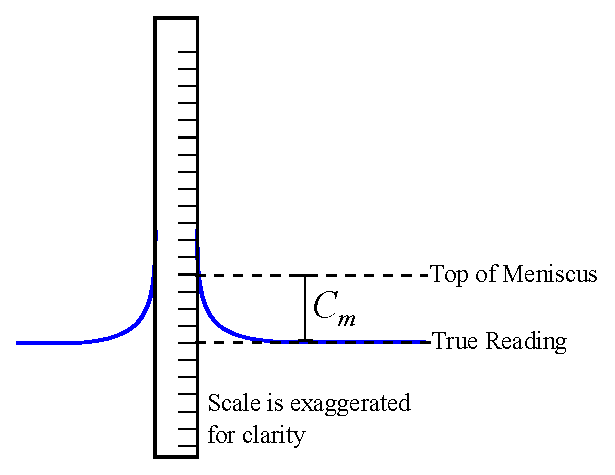
\includegraphics[width=0.5\textwidth]{meniscus.eps}
    \caption{Schematic of true and top of meniscus reading locations. The resulting correction factor, $C_m$, is shown as the difference between the two readings.}
    \label{fig:meniscus}
\end{figure}

\subsubsection*{Preparation Checklist}
\begin{itemize}
    \item Weigh moist soil sample
    \item Weigh a second sample to oven dry for moisture content
    \item If needed, weigh and add the dispersant
    \item Determine the meniscus correction factor for the hydrometer
\end{itemize}

\subsubsection{Execution}
The ASTM D7928 test procedure is relatively straightforward. The precise details are described in ASTM D7928 \S11. For this laboratory exercise, we are using the referee stirring apparatus (i.e. milkshake-style blender) and referee agitator. The procedure involves an overnight rest period for the slurry to completely deflocculate. We will not employ the overnight conditioning period for this laboratory exercise.

The previously weighed sample is blended using a milkshake-style blender to homogenize and deflocculate the slurry. The blender cup should contain all of the weighed sample and enough of the test water, with or without the dispersant, depending on the sample, to fill the cup about halfway. The soil slurry should be blended for about 1 minute.

After blending, transfer the slurry to the sedimentation container. To get 100\% of the slurry out of the blender cup, use a squirt bottle containing the test water, with or without the dispersant, depending on the sample, to rinse out the cup completely. Then fill the sedimentation container up to the 1000 mL line with the test water, with or without the dispersant, depending on the sample. You will then use the agitator to homogenize the slurry. You will start with the agitator near the bottom of the sedimentation container, using an smooth up and down motion. Watch the accompanying video to see this process more clearly. Agitate the solution for about 1 minute.

At this point, the slurry would normally be left to condition overnight. However, we will continue with the test procedure as described in ASTM D7928, resuming at \S11.7.2. As soon as you remove the agitator from the sedimentation container, start a timer. Your first reading with the hydrometer will occur at the 1 minute mark, so ensure you have everything ready.

Approximately 20 seconds before the 1 minute mark, slowly guide the hydrometer into the soil solution. Be careful and do not allow the hydrometer to spin or bob. Ideally, you lower the hydrometer in the soil solution and when you notice it is neutrally buoyant, carefully release your grip. You want to have the hydrometer stabilized so that precisely at the 1 minute mark, you can take a reading. You will read the hydrometer from the top of the meniscus as described earlier.

Once you have obtained your reading, slowly and carefully remove the hydrometer. It should take you about 15 seconds to remove it from the soil solution. You are trying to minimize the disturbance of the solution and do not want to affect the particles from settling out. Once the hydrometer is removed, measure the temperature of the soil solution using the provided thermometer. The remaining times at which you must take a reading are listed in ASTM D7928 \S11.8. Note that the next time is at 2 minutes from the point the agitator left the soil solution and no, you cannot leave the hydrometer in the soil sedimentation container to take that reading.

Each time you remove the hydrometer, you should rinse it off, dry it completely, and return it to the reference sedimentation container. This reference container only has water or water with the dispersant in it. The appendix\footnote{Not the annex, but appendix. They are both at the end.} of ASTM D7928 has two examples of data collection sheets that might be useful references for designing your own to record the experimental data. Namely, X1.1, X1.2, and X1.7 provide good references.

After the last reading, the slurry will be rinsed through a \#200 sieve. The material retained on the \#200 sieve will be oven dried and then weighed. This data will be provided to you.

\subsubsection*{Execution Checklist}
\begin{itemize}
    \item Record the hydrometer reading at the specified times
    \item Record the soil solution temperature at the specified times
\end{itemize}

\subsubsection{Analysis}
The analysis of the hydrometer data is more involved than the sieve analysis. The calculations are described in detail in ASTM D7928 \S12. You should go step by step and create a spreadsheet to perform the calculations. To help you setup your spreadsheet, the following flowchart (Fig. \ref{fig:D7928flowchart}) describes the calculation process for each reading. After you setup your spreadsheet, it is recommended that you check your calculations with the two examples provided in the appendix (Fig. X1.1 and X1.2).

\begin{figure}[H]
\centering
    \begin{tikzpicture}[node distance=3cm]
        \node (eq4) [startstop] {Eq. 4};
        \node (eq7) [startstop, right of=eq4] {Eq. 7};
        \node (eq9) [startstop, right of=eq7] {Eq. 9};
        \node (eq10) [startstop, right of=eq9] {Eq. 10};
        \node (eq11) [startstop, right of=eq10] {Eq. 11};
        \draw [arrow] (eq4) -- (eq7);
        \draw [arrow] (eq7) -- (eq9);
        \draw [arrow] (eq9) -- (eq10);
        \draw [arrow] (eq10) -- (eq11);
    \end{tikzpicture}
    \caption{Flowchart of hydrometer calculations referencing the equation numbers in ASTM D7928. This flowchart uses the equations for the 152H hydrometer used in lab. Other equations are neccessary if a 151H hydrometer was used.}
    \label{fig:D7928flowchart}
\end{figure}

The second part is incorporating the hydrometer readings into your previous sieve analysis. If you notice, the hydrometer particle size analysis ``starts'' at the \#200. It combines all the particles that are larger than 75 $\mu$m together. We cannot directly add the particle size distribution from the hydrometer to the end of the sieve analysis and call it a day. We must put the data in context of the entire gradation.

The easiest way to explain this is to go through an example. A hydrometer dataset is shown in Table \ref{tab:hydrometer}. Let's also use the gradation shown in Table \ref{tab:FM}. There is 3\% passing the \#200 sieve. But wait, we have 56\% finer as the first value in our hydrometer analysis! We need to normalize the hydrometer values to the amount that passed the \#200 sieve in our sieve analysis. For instance, in the hydrometer analysis, we have 56\% passing the 0.0450 mm size. In the context of the whole gradation, that is 56\% of 3\%, which is 1.68\%. That means at the 0.0450 mm size, we have 1.68\% passing in the context of the whole gradation. We continue the trend for all the measured particle sizes from the hydrometer analysis. 

\begin{table}[H]
    \centering
        \caption{Example dataset from hydrometer testing.}
    \label{tab:hydrometer}
    \begin{tabular}{cc}
\hline
$D$, mm & Mass \% Finer, $N_m$ \\ \hline
0.0450 & 56\\
0.0331 & 32\\
0.0261 & 21\\
0.0174 & 14\\
0.0120 & 11\\
0.0099 & 9\\
0.0071 & 5\\
0.0028 & 4\\
0.0013 & 3\\ \hline
\end{tabular}
\end{table}

\subsubsection*{Analysis Checklist}
\begin{itemize}
    \item Calculate particle sizes from hydrometer readings and associated mass percent finer values
    \item Incorporate the hydrometer values into the overall gradation data
\end{itemize}

\subsection{Summary}
We have successfully planned, executed, and analyzed the results of a hydrometer analysis on two different materials using ASTM D7928. This test procedures provides critical information about the clay and silt components of a soil and can allow us to make important design decisions. Although there are more accurate methods to determine small particle sizes, the hydrometer test method is straightforward, simple, and cheap.

%\section*{References}
%\addcontentsline{toc}{section}{References}
%\bibliographystyle{techpubs}
%\bibliography{References}

%%%%%%%%%%%%%%%%%%%%%%%%%%%%%%%%%%%%%%%%%%%%%%%%%%%%%%%%%%%%%%%%%%%%
%   Please use the techpubs BibTeX style when compiling bibliography, or follow the instructions on tinyurl.com/techpubsnist to format your .bib / .bbl file appropriately.
%%%%%%%%%%%%%%%%%%%%%%%%%%%%%%%%%%%%%%%%%%%%%%%%%%%%%%%%%%%%%%%%%%%%
\pagebreak

\section*{Appendix A: Example Gradation Worksheet}
\label{AppendixA}
\addcontentsline{toc}{section}{Appendix A: Example Gradation Worksheet}
\begin{center}
    \includegraphics[width=1\linewidth]{Example_Sieve_Analysis_Worksheet.eps}
\end{center}

\pagebreak
\section*{Appendix B: Change Log}
\addcontentsline{toc}{section}{Appendix B: Change Log}
This document was originally created on April 9, 2020. Any changes will be documented in this appendix.

\end{document}
%%%%%%%%%%%%%%%%%%%%%%%%%%%%%%%%%%%%%%%%%%%%%%%%%%%%%%%%%%%%%%%%%%%%
%   When referring to references in the text parenthetically, 
%	use the form “[1].” For example, “As Jones and Smith have shown [1];”
%	 however, when a reference is referred to non-parenthetically, use the form 
%	“. . . Ref. [1] . . .” (except at the beginning of a sentence where
%	“Reference [1] . . .” is the correct form).
%%%%%%%%%%%%%%%%%%%%%%%%%%%%%%%%%%%%%%%%%%%%%%%%%%%%%%%%%%%%%%%%%%%%

%%%%%%%%%%%%%%%%%%%%%%%%%%%%%%%%%%%%%%%%%%%%%%%%%%%%%%%%%%%%%%%%%%%%
%   Section references are “Sec. X”.
% 	“Section X” is used at beginning of sentence. 
%%%%%%%%%%%%%%%%%%%%%%%%%%%%%%%%%%%%%%%%%%%%%%%%%%%%%%%%%%%%%%%%%%%%

%%%%%%%%%%%%%%%%%%%%%%%%%%%%%%%%%%%%%%%%%%%%%%%%%%%%%%%%%%%%%%%%%%%%
%   Equation references are “Eq. (X)”.
% 	“Equation (1) is used at beginning of sentence.
%	Equations are numbered (#) on the right, per the standard LaTeX format
%%%%%%%%%%%%%%%%%%%%%%%%%%%%%%%%%%%%%%%%%%%%%%%%%%%%%%%%%%%%%%%%%%%%

%%%%%%%%%%%%%%%%%%%%%%%%%%%%%%%%%%%%%%%%%%%%%%%%%%%%%%%%%%%%%%%%%%%%
%   Tables should appear after they are mentioned in the text. 
%	Superscripted letters (a, b, c, etc.) should be used for table footnotes.
%%%%%%%%%%%%%%%%%%%%%%%%%%%%%%%%%%%%%%%%%%%%%%%%%%%%%%%%%%%%%%%%%%%%

%%%%%%%%%%%%%%%%%%%%%%%%%%%%%%%%%%%%%%%%%%%%%%%%%%%%%%%%%%%%%%%%%%%%
%   Figure references are “Fig. X”.
% 	“Figure X” is used at beginning of sentence. 
% 	Figures should appear after they are mentioned in the text.
%	Figures must have embedded alternate text or “alt text” in order 
%	to comply with Section 508 accessibility standards. 
%%%%%%%%%%%%%%%%%%%%%%%%%%%%%%%%%%%%%%%%%%%%%%%%%%%%%%%%%%%%%%%%%%%%